\documentclass{article}

\usepackage{fontspec}
\usepackage{fullpage}
\usepackage{multicol}
\usepackage{multirow}
\usepackage{tikz}

\begin{document}

\newfontfamily\swfill{SuttonSignWritingFill.ttf}
\newfontfamily\swline{SuttonSignWritingLine.ttf}
\newcommand{\bul}{\hfil$\bullet$&}
\renewenvironment{glossary}{\begin{multicols}{5}\begin{center}}{\end{center}\end{multicols}}
\setcounter{secnumdepth}{0}
\setlength{\columnseprule}{1pt}

\section{Supplement For Lesson 3}

\begin{center}
\it
Objectives inspired by, vocabulary transcribed from, and sentences and story by Bill Vicars.

Handshape photos by Adam Frost.

No endorsement implied nor given by either.
\end{center}

\subsection{Objectives}

\begin{tabular}{p{1cm}p{14cm}}
\bul I have completed the objectives for this lesson.\\
\bul I am able to read the numbers 11--20.\\
\bul I am able to demonstrate how SignWriting handles sign parameters.\\
\bul I am able to show the meaning and form of the symbol groups in the movement category.\\
\bul I am able to write and sign the fingershapes.\\
\bul I understand the types of handshapes in Symbol Groups four and five.\\
\bul I am able to draw the circle palmshape in all forms.\\
\bul I am able to draw and demonstrate what fill two means.\\
\bul I am able to read, write, and sign the ASL handshapes in symbol group two.\\
\bul I am able to recognize the vocabulary for lesson.\\
\bul I am able to read the practice sentences for this lesson.\\
\bul I am able to read the practice story for this lesson.\\
\end{tabular}

\subsection{The Numbers 11 through 20}

You'll notice that we show these different than your practice sentences.
That was because it was ``numbers'', these are different because they are ``text''.

\begin{center}
\begin{tabular}{*{5}{c}}
\textbf{11}&\textbf{12}&\textbf{13}&\textbf{14}&\textbf{15}\\
B512x520S10000489x490S21d00494x480&
B509x521S10e00491x491S21d00491x480&
B513x519S22114487x481S12d00489x489&
B513x515S14700493x493S22114487x486&
B513x518S22114487x483S15d00494x491\\
\textbf{16}&\textbf{17}&\textbf{18}&\textbf{19}&\textbf{20}\\
B520x522S18700502x492S2e00e480x479&
B522x522S1a500501x494S2e00e478x478&
B523x522S1bb00502x492S2e00e478x479&
B524x522S1ce00502x490S2e00e477x479&
B517x513S22114484x488S1f420488x498\\
\end{tabular}
\end{center}

\subsection{Sign Parameters}

One of the strengths of SignWriting is that it actually handles each of these parameters.
Let's see how the slightly longer list of five parameters is handled.

\begin{center}
\begin{tabular}{rcl}
\textbf{Parameter}&\textbf{How Handled}&\textbf{Examples}\\
Handshape         &Category 1       &B508x515S10000493x485 B508x515S10f00492x485\\
Location          &Relative location&B518x518S2ff00482x483S20500495x469S14c10468x453 B518x535S2ff00482x483S20500494x520S14c10471x504\\
Movement          &Category 2       &B507x508S22a00494x493 B507x508S26500493x493\\
Orientation       &Fill \& Rotation &B508x515S10000493x485 B508x515S10010493x485 B508x515S10040493x485\\
Non-manual Markers&Category 3       &B518x518S30a00482x483 B518x518S30c00482x483\\
\end{tabular}
\end{center}

\subsection{The Movement Category}

The second category is called ``Movement'' and has ten symbols that you will learn in future lessons.
The symbol groups can be thought of as three groups of ten, and these are the second ten.

\begin{center}
\begin{tabular}{ccp{21mm}c@{\hskip 5mm}ccp{21mm}c}
\textbf{Symbol}&&&&\textbf{Symbol}\\
\textbf{Group}&\textbf{Name}&\textbf{Meaning}&\textbf{Example}&\textbf{Group}&\textbf{Name}&\textbf{Meaning}&\textbf{Example}\\
\textbf{11}&Contact    &How do they touch?&B505x506S20500495x495&\textbf{12}&Finger    &What are fingers doing? &B504x504S21600496x496\\
\textbf{13}&Wall       &Vertical.         &B507x508S22a00494x493&\textbf{14}&Diagonal  &Wall and floor together.&B507x511S25500494x489\\
\textbf{15}&Floor      &Horizontal.       &B507x508S26500493x493&\textbf{16}&Curve Wall&Vertical arcs.          &B506x511S28800494x489\\
\textbf{17}&Hit Wall   &Both up and down. &B509x512S2a600492x489&\textbf{18}&Hit Floor &Back and forth.         &B510x512S2b700491x489\\
\textbf{19}&Curve Floor&Horizontal arcs.  &B511x505S2d500489x496&\textbf{20}&Circle    &All the way around.     &B512x514S2e300489x487\\
\end{tabular}
\end{center}

You will need to be able to recite these eventually.
For now, just be aware of them.
We will learn the order in future lessons.

\subsection{Fingershapes}

After you have drawn a palmshape, you will need to decorate it with fingers in one of several forms.
They are, from most up to the most at the side.

\begin{center}
\begin{tabular}{cccc}
Normal or Hinged (straight)&B500x500S10000500x500 B508x515S10b10492x486&Cup      &B500x500S10a00500x500\\
Bent                       &B500x500S10600500x500                      &Bumped   &B508x510S10900493x490\\
Group Bent                 &B500x500S1e600500x500                      &Group Cup&B500x500S1ed00500x500\\
Group Straight             &B500x500S1ef00500x500\\
\end{tabular}
\end{center}

The thumb is either cup or straight and is drawn last.

\subsection{Symbol Groups Four and Five}

The fourth Symbol Group we informally call four though it's official name is ``Four Fingers''.
Symbol Group Four Fingers (Four) have all the handshapes with four fingers extended and thumb held close.

The fifth Symbol Group we informally call five, though it's official name is ``Five Fingers''.
Symbol Group Five Fingers (Five) have four types of symbols:
first are symbols with all five fingers specified,
second are symbols with four fingers but the thumb held loosely (and therefore missing) or extended.
third are symbols with four fingers acting as a group but with the thumb held loosely or extended.
and fourth are palmshapes that aren't fist.
That may seem like an eclectic mix, but in all cases all five fingers are doing something.
The reason that the fist palmshape is not part of this symbol group is because when making a fist the thumb is held to the side, so it goes in the thumb symbol group.

Before you can consider this lesson complete, you need to be able to list off the symbol grops as:
``one, two, three, four, five''.

\subsection{The Circle Palmshape}

\begin{center}
\begin{tabular}{r*{6}{c}}
&\textbf{Fill 1}&\textbf{Fill 2}&\textbf{Fill 3}&\textbf{Fill 4}&\textbf{Fill 5}&\textbf{Fill 6}\\
\multirow{2}{*}{\textbf{Right}}&
B508x508S17600492x492&
B508x508S17610492x492&
B508x508S17620492x492&
B508x508S17630492x492&
B508x508S17640492x492&
B508x508S17650492x492\\
&
\tikz{\draw(0,0)circle(7pt);}&
\tikz{\draw(0,0)circle(7pt);\draw(0,7pt)--(0,-7pt);\draw(0,7pt)--(5pt,-5pt);\draw(0,-7pt)--(5pt,5pt);}&
\tikz{\draw(0,0)circle(7pt);\draw(-5pt,5pt)--(5pt,-5pt);\draw(5pt,5pt)--(-5pt,-5pt);}&
\tikz{\draw(0,0)circle(7pt);\draw(-10pt,3pt)--(10pt,3pt);}&
\tikz{\draw(0,0)circle(7pt);\draw(0,7pt)--(0,-7pt);\draw(0,7pt)--(5pt,-5pt);\draw(0,-7pt)--(5pt,5pt);\draw(-10pt,3pt)--(10pt,3pt);}&
\tikz{\draw(0,0)circle(7pt);\draw(-5pt,5pt)--(5pt,-5pt);\draw(5pt,5pt)--(-5pt,-5pt);\draw(-10pt,3pt)--(10pt,3pt);}\\
\textbf{Left}&
B508x508S17608492x492&
B508x508S17618492x492&
B508x508S17628492x492&
B508x508S17638492x492&
B508x508S17648492x492&
B508x508S17658492x492\\
\end{tabular}
\end{center}

\subsection{The Second Fill}

\subsubsection{Hand Symbols}

\begin{center}
B508x515S10010493x485 B508x515S10e10493x485 B512x515S11e10489x485
\end{center}

Any symbol drawn in the second fill means that the signer's thumb is facing the signer.
For all the hand symbols, the empty portion represents the signer's palm and the filled portion represents the back of the hand.
So for fill two, if the hand was open you would be able to see your palm and the back of your hand --- leaving fill two a half-full symbol.

\subsubsection{Movement Symbols}

\begin{center}
B508x515S22b10492x485 B508x515S25610492x485 B508x515S26610492x485
\end{center}

Any symbol drawn in the second fill means that the left hand is doing the movement, so these movements are all left hand movements.

\subsubsection{Everything Else}

\begin{center}
B506x504S2f710494x497 B518x518S30a10482x483 B537x504S38710463x496
\end{center}

The fills for other categories tend to be a bit more variable.
Here we have an alternate form of fast, right eyebrow raised, and fast comma.

\subsection{ASL Handshapes From Symbol Group Two}

The six handshapes in Symbol Group Two used by ASL in order are:
{\bf
Index Middle;
Index Middle Bent;
Index Middle Unit;
Index Middle Unit, Cup;
Index Middle Unit, Hinge;
and Index Middle Cross.
}

\subsubsection{The Index Middle Handshape}

\begin{center}
\begin{tabular}{r*{6}{c}}
&\textbf{Fill 1}&\textbf{Fill 2}&\textbf{Fill 3}&\textbf{Fill 4}&\textbf{Fill 5}&\textbf{Fill 6}\\
\multirow{2}{*}{\textbf{Right}}&
B508x515S10e00493x485&
B508x515S10e10493x485&
B508x515S10e20493x485&
B508x515S10e30493x485&
B508x515S10e40493x485&
B508x515S10e50493x485\\
&
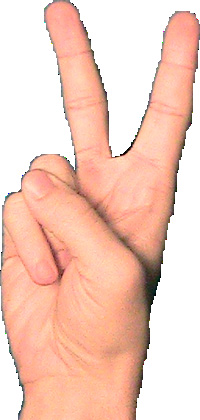
\includegraphics[scale=0.1]{images/02-01-1.jpg}&
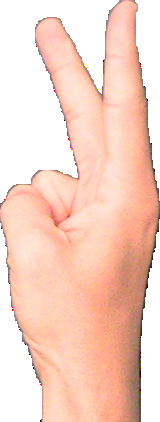
\includegraphics[scale=0.1]{images/02-01-2.jpg}&
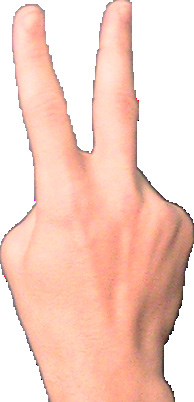
\includegraphics[scale=0.1]{images/02-01-3.jpg}&
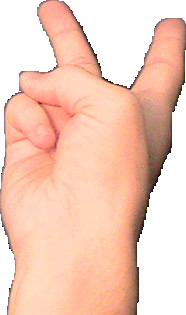
\includegraphics[scale=0.1]{images/02-01-4.jpg}&
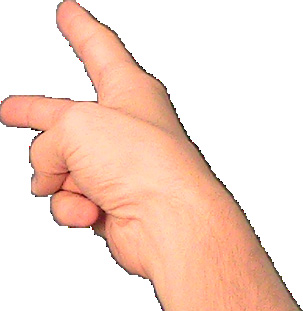
\includegraphics[scale=0.1]{images/02-01-5.jpg}&
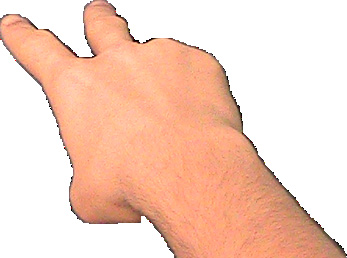
\includegraphics[scale=0.1]{images/02-01-6.jpg}\\
\textbf{Left}&
B508x515S10e08493x485&
B508x515S10e18493x485&
B508x515S10e28493x485&
B508x515S10e38493x485&
B508x515S10e48493x485&
B508x515S10e58493x485\\
\end{tabular}
\end{center}

\subsection{The Index Middle Bent Handshape}

\begin{center}
\begin{tabular}{r*{6}{c}}
&\textbf{Fill 1}&\textbf{Fill 2}&\textbf{Fill 3}&\textbf{Fill 4}&\textbf{Fill 5}&\textbf{Fill 6}\\
\multirow{2}{*}{\textbf{Right}}&
B508x514S11000493x487&
B508x514S11010493x487&
B508x514S11020493x487&
B508x514S11030493x487&
B508x514S11040493x487&
B508x514S11050493x487\\
&
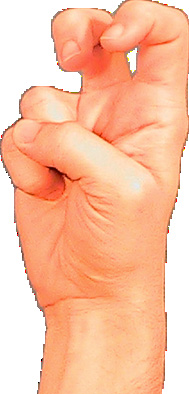
\includegraphics[scale=0.1]{images/02-02-1.jpg}&
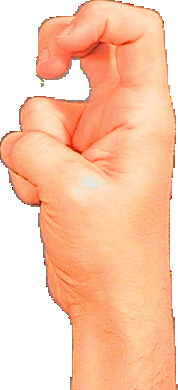
\includegraphics[scale=0.1]{images/02-02-2.jpg}&
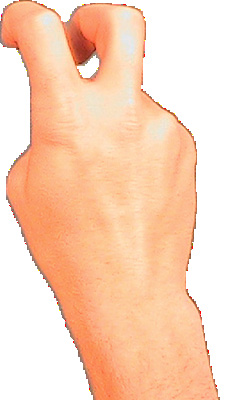
\includegraphics[scale=0.1]{images/02-02-3.jpg}&
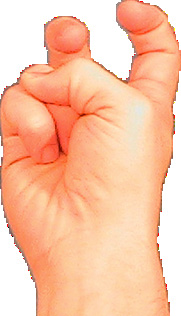
\includegraphics[scale=0.1]{images/02-02-4.jpg}&
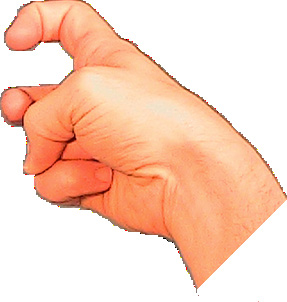
\includegraphics[scale=0.1]{images/02-02-5.jpg}&
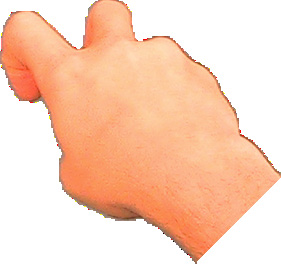
\includegraphics[scale=0.1]{images/02-02-6.jpg}\\
\textbf{Left}&
B508x514S11008493x487&
B508x514S11018493x487&
B508x514S11028493x487&
B508x514S11038493x487&
B508x514S11048493x487&
B508x514S11058493x487\\
\end{tabular}
\end{center}

\subsubsection{The Index Middle Unit Handshape}

\begin{center}
\begin{tabular}{r*{6}{c}}
&\textbf{Fill 1}&\textbf{Fill 2}&\textbf{Fill 3}&\textbf{Fill 4}&\textbf{Fill 5}&\textbf{Fill 6}\\
\multirow{2}{*}{\textbf{Right}}&
B508x515S11500493x485&
B508x515S11510493x485&
B508x515S11520493x485&
B508x515S11530493x485&
B508x515S11540493x485&
B508x515S11550493x485\\
&
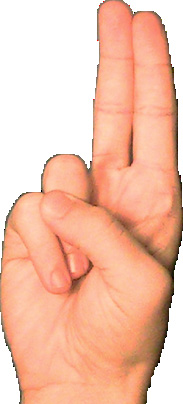
\includegraphics[scale=0.1]{images/02-03-1.jpg}&
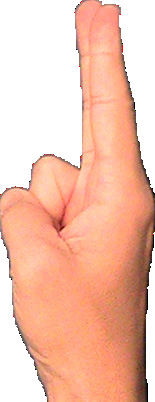
\includegraphics[scale=0.1]{images/02-03-2.jpg}&
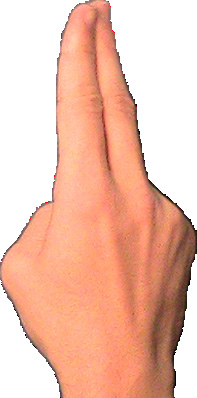
\includegraphics[scale=0.1]{images/02-03-3.jpg}&
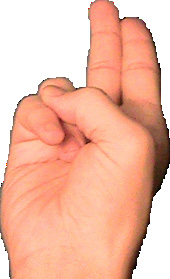
\includegraphics[scale=0.1]{images/02-03-4.jpg}&
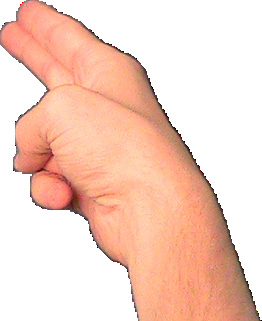
\includegraphics[scale=0.1]{images/02-03-5.jpg}&
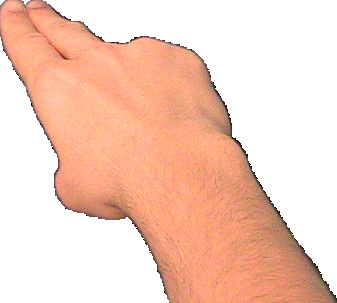
\includegraphics[scale=0.1]{images/02-03-6.jpg}\\
\textbf{Left}&
B508x515S11508493x485&
B508x515S11518493x485&
B508x515S11528493x485&
B508x515S11538493x485&
B508x515S11548493x485&
B508x515S11558493x485\\
\end{tabular}
\end{center}

\subsubsection{The Index Middle Unit, Cup Handshape}

\begin{center}
\begin{tabular}{r*{6}{c}}
&\textbf{Fill 1}&\textbf{Fill 2}&\textbf{Fill 3}&\textbf{Fill 4}&\textbf{Fill 5}&\textbf{Fill 6}\\
\multirow{2}{*}{\textbf{Right}}&
B508x514S11800493x487&
B508x514S11810493x487&
B508x514S11820493x487&
B508x514S11830493x487&
B508x514S11840493x487&
B508x514S11850493x487\\
&
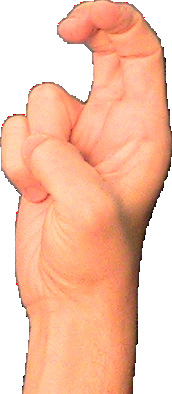
\includegraphics[scale=0.1]{images/02-04-1.jpg}&
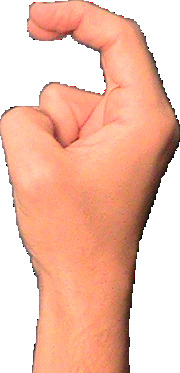
\includegraphics[scale=0.1]{images/02-04-2.jpg}&
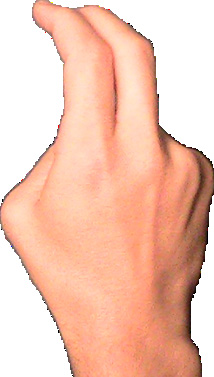
\includegraphics[scale=0.1]{images/02-04-3.jpg}&
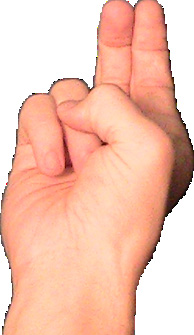
\includegraphics[scale=0.1]{images/02-04-4.jpg}&
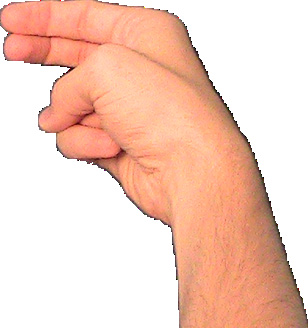
\includegraphics[scale=0.1]{images/02-04-5.jpg}&
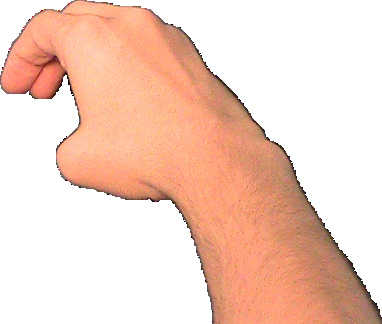
\includegraphics[scale=0.1]{images/02-04-6.jpg}\\
\textbf{Left}&
B508x514S11808493x487&
B508x514S11818493x487&
B508x514S11828493x487&
B508x514S11838493x487&
B508x514S11848493x487&
B508x514S11858493x487\\
\end{tabular}
\end{center}

\subsubsection{The Index Middle Unit, Hinge Handshape}

\begin{center}
\begin{tabular}{r*{6}{c}}
&\textbf{Fill 1}&\textbf{Fill 2}&\textbf{Fill 3}&\textbf{Fill 4}&\textbf{Fill 5}&\textbf{Fill 6}\\
\multirow{2}{*}{\textbf{Right}}&
B509x513S11900492x488&
B509x513S11910492x488&
B509x513S11920492x488&
B509x513S11930492x488&
B509x513S11940492x488&
B509x513S11950492x488\\
&
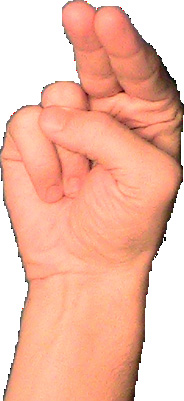
\includegraphics[scale=0.1]{images/02-05-1.jpg}&
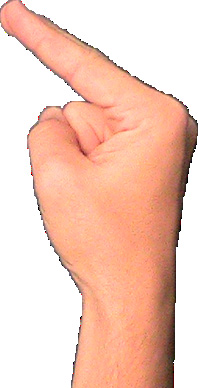
\includegraphics[scale=0.1]{images/02-05-2.jpg}&
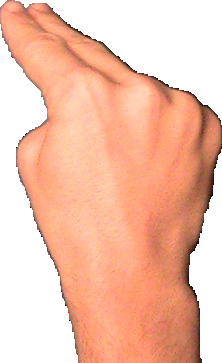
\includegraphics[scale=0.1]{images/02-05-3.jpg}&
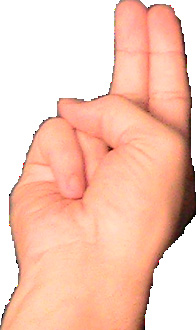
\includegraphics[scale=0.1]{images/02-05-4.jpg}&
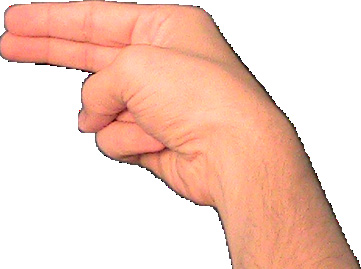
\includegraphics[scale=0.1]{images/02-05-5.jpg}&
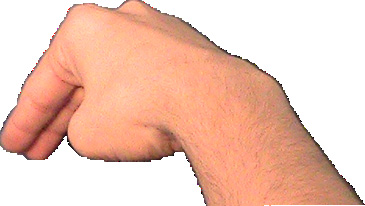
\includegraphics[scale=0.1]{images/02-05-6.jpg}\\
\textbf{Left}&
B509x513S11908492x488&
B509x513S11918492x488&
B509x513S11928492x488&
B509x513S11938492x488&
B509x513S11948492x488&
B509x513S11958492x488\\
\end{tabular}
\end{center}

\subsubsection{The Index Middle Cross Handshape}

\begin{center}
\begin{tabular}{r*{6}{c}}
&\textbf{Fill 1}&\textbf{Fill 2}&\textbf{Fill 3}&\textbf{Fill 4}&\textbf{Fill 5}&\textbf{Fill 6}\\
\multirow{2}{*}{\textbf{Right}}&
B508x515S11a00493x485&
B508x515S11a10493x485&
B508x515S11a20493x485&
B508x515S11a30493x485&
B508x515S11a40493x485&
B508x515S11a50493x485\\
&
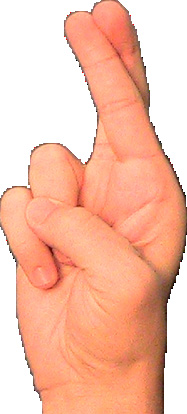
\includegraphics[scale=0.1]{images/02-06-1.jpg}&
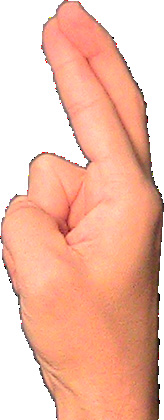
\includegraphics[scale=0.1]{images/02-06-2.jpg}&
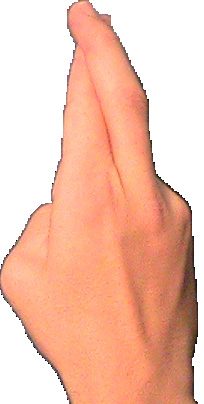
\includegraphics[scale=0.1]{images/02-06-3.jpg}&
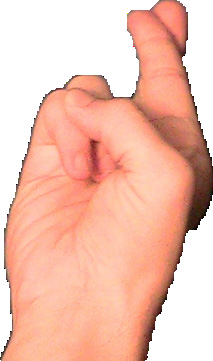
\includegraphics[scale=0.1]{images/02-06-4.jpg}&
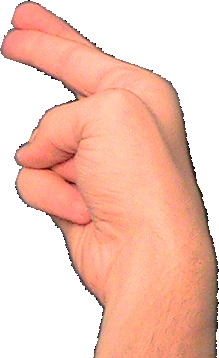
\includegraphics[scale=0.1]{images/02-06-5.jpg}&
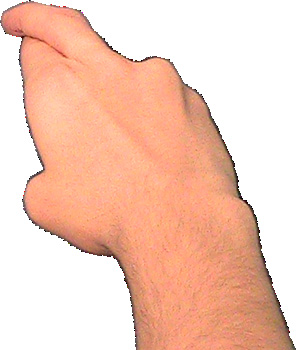
\includegraphics[scale=0.1]{images/02-06-6.jpg}\\
\textbf{Left}&
B508x515S11a08493x485&
B508x515S11a18493x485&
B508x515S11a28493x485&
B508x515S11a38493x485&
B508x515S11a48493x485&
B508x515S11a58493x485\\
\end{tabular}
\end{center}

\subsection{Vocabulary}

\begin{glossary}

\textbf{11}\\
AS10000S21d00M512x520S10000489x490S21d00494x480

\textbf{12}\\
AS10e00S21d00M509x521S10e00491x491S21d00491x480

\textbf{13}\\
AS12d00S22114M513x519S22114487x481S12d00489x489

\textbf{14}\\
AS14700S22114M513x515S14700493x493S22114487x486

\textbf{15}\\
AS15d00S22114M513x518S22114487x483S15d00494x491

\textbf{16}\\
AS18700S2e00eM520x522S18700502x492S2e00e480x479

\textbf{17}\\
AS1a500S2e00eM522x522S1a500501x494S2e00e478x478

\textbf{18}\\
AS1bb00S2e00eM523x522S1bb00502x492S2e00e478x479

\textbf{19}\\
AS1ce00S2e00eM524x522S1ce00502x490S2e00e477x479

\textbf{20}\\
AS1f420S22114M517x513S22114484x488S1f420488x498

\textbf{academic}\\
AS15a5fS15a39S20600M512x519S15a39489x496S15a5f488x496S20600489x482

\textbf{all}\\
AS15a20S2e700S15d01S15d09S20500M520x551S2e700504x483S15d09481x520S20500505x513S15d01493x528S15a20508x450

\textbf{ask}\\
AS10000S26500S10600M508x543S10000492x458S26500493x494S10600493x517

\textbf{bad}\\
AS15a00S22b04S15a51S2ff00M518x602S2ff00482x483S22b04494x540S15a00495x507S15a51494x579

\textbf{bathroom}\\
AS1fb20S27106M518x520S1fb20482x490S27106503x480

\textbf{best}\\
AS15a01S28807S1f502S2ff00M542x543S2ff00482x483S15a01495x520S28807521x506S1f502527x478

\textbf{better}\\
AS15a01S28806S1f502S2ff00M555x543S2ff00482x483S15a01495x520S28806519x530S1f502540x505

\textbf{big}\\
AS1e110S1e118S26606S26612M539x527S1e110506x473S1e118470x473S26606509x511S26612462x511

\textbf{brain}\\(think)
AS10011S20500S2ff00M539x519S2ff00482x483S10011518x489S20500510x474

\textbf{city}\\
AS15a11S15a19S20500S26526S15a11S15a19S20500M562x520S20500458x480S15a19439x494S15a11463x494S26526496x498S15a19514x497S15a11539x496S20500533x480

\textbf{class}\\
AS16d10S16d18S2df06S2df1eS2fb00M527x528S16d10509x508S16d18473x508S2df06507x479S2df1e473x480S2fb00493x473

\textbf{come}\\
AS10001S10009S2b734S2b745S2fb00M534x532S10001513x469S10009467x469S2b734507x513S2b745481x513S2fb00496x500

\textbf{don't}\\
AS15a51S15a59S26606S26612M543x515S15a51480x486S15a59494x487S26606513x499S26612458x499

\textbf{don't like}\\
AS14c52S2d200S1bb02M516x538S1bb02488x517S14c52484x463S2d200490x490

\textbf{family}\\
AS1ce20S1ce28S2df06S2df1eS2fb00M524x534S1ce20502x504S1ce28477x504S2df06502x476S2df1e478x476S2fb00494x467

\textbf{favorite}\\
AS1c507S20600S2ff00M540x543S1c507499x518S20600518x508S2ff00482x483

\textbf{fine}\\
AS14c10S20600M524x516S14c10477x485S20600502x496

\textbf{from}\\
AS10041S10028S20500S26505S10641M535x542S10028465x470S26505496x499S10041477x471S20500470x458S10641512x514

\textbf{go}\\
AS10018S10018S2882aM525x526S10018476x477S10018497x496S2882a503x475

\textbf{good}\\
AS15a00S22a04S15a3fS15a39S2ff00M518x585S2ff00482x483S15a00494x509S22a04494x539S15a39479x557S15a3f494x562

\textbf{grow up}\\
AS15a50S22b00M508x532S22b00492x502S15a50494x468

\textbf{have to}\\
AS10620S22e04M512x524S10620489x476S22e04495x506

\textbf{here}\\
AS15a30S15a30S2e508S2e510S2fb04M532x535S15a30475x466S15a30512x466S2fb04494x529S2e510468x498S2e508509x498

\textbf{house}\\
AS15a11S15a19S20500S23804S2381cS2fb04M525x539S15a11502x476S15a19476x476S20500495x462S23904505x501S2391c477x501S2fb04494x533

\textbf{inquire}\\
AS10000S26500S10600M508x543S10000492x458S26500493x494S10600493x517

\textbf{mind}\\
AS10011S20500S2ff00M539x519S2ff00482x483S10011518x489S20500510x474

\textbf{more}\\
AS18510S18518S20500M526x517S18510501x502S18518475x502S20500495x484

\textbf{must}\\
AS10620S22e04M512x524S10620489x476S22e04495x506

\textbf{need}\\
AS10620S22e04M512x524S10620489x476S22e04495x506

\textbf{not}\\
AS1f540S20e00S26500S2ff00M534x543S2ff00482x483S26500520x505S20e00521x526S1f540494x519

\textbf{ought to}\\
AS10620S23004M514x524S10620486x476S23004489x506

\textbf{prefer}\\
AS1c507S20600S2ff00M540x543S1c507499x518S20600518x508S2ff00482x483

\textbf{raised}\\
AS15a50S22b00M508x532S22b00492x502S15a50494x468

\textbf{request}\\
AS15a10S15a18S2b724M513x531S15a10501x504S15a18488x504S2b724494x470

\textbf{restroom}\\
AS1fb20S27106M518x520S1fb20482x490S27106503x480

\textbf{school}\\
AS15a5fS15a39S20600M512x519S15a39489x496S15a5f488x496S20600489x482

\textbf{should}\\
AS10620S23004M514x524S10620486x476S23004489x506

\textbf{small}\\
AS15a10S15a18S26502S26516S2fb00M526x528S15a18476x472S15a10514x472S2fb00492x504S26502511x513S26516474x514

\textbf{so so}\\
AS14c50S2a508M512x535S14c50488x466S2a508490x502

\textbf{sort of}\\
AS14c50S2a508M512x535S14c50488x466S2a508490x502

\textbf{think}\\
AS10011S20500S2ff00M539x519S2ff00482x483S10011518x489S20500510x474

\textbf{think about}\\
AS10011S20600S2ff00M540x520S2ff00482x483S10011519x490S20600511x474

\textbf{toilet}\\
AS1fb20S27106M518x520S1fb20482x490S27106503x480

\textbf{want}\\
AS14c30S14c38S26524S15030S15038M534x543S14c30507x457S14c38469x458S15030508x512S15038467x511S26524493x493

\textbf{whole}\\
AS15a20S2e700S15d01S15d09S20500M520x551S2e700504x483S15d09481x520S20500505x513S15d01493x528S15a20508x450

\textbf{wonder}\\
AS10011S20600S2ff00M540x520S2ff00482x483S10011519x490S20600511x474

\end{glossary}

\subsection{Practice Sheet 3.A}

\begin{multicols}{5}
\begin{center}

M508x515S10000493x485 % 1
M536x504S38800464x496 % .
M528x526S10000473x496S26507494x495S10600513x474 % ask them
M522x525S11541498x491S11549479x498S20600489x476 % name
M536x504S38800464x496 % .
\vfil
\columnbreak

M508x515S10e00493x485 % 2
M536x504S38800464x496 % .
M510x523S10040495x493S26500491x478 % you
M520x522S1f502505x498S1f50a480x498S22a20493x478 % live
M518x518S30c00482x483 % \?
M562x520S20500458x480S15a19439x494S15a11463x494S26526496x498S15a19514x497S15a11539x496S20500533x480 % city
M536x507S38900464x493 % ?
\vfil
\columnbreak

M512x515S11e00489x485 % 3
M536x504S38800464x496 % .
M518x518S30a00482x483 % y/n
M510x523S10040495x493S26500491x478 % you
M516x540S1bb02488x461S14c02484x517S20e00499x502S26500499x483 % like
M543x567S15a37482x526S14c51500x541S22c00520x503S20500512x467S18510518x482S2ff00482x483S20500488x533 % learn
M523x535S2ea48483x510S10011502x466S2ea04508x500S10019477x475 % sign (as in ``signing'')
M536x507S38900464x493 % ?
\vfil
\columnbreak

M511x516S14400489x485 % 4
M536x504S38800464x496 % .
M518x518S30a00482x483 % y/n
M507x523S15a28494x496S26500493x477 % your
M525x539S15a11502x476S15a19476x476S20500495x462S23904505x501S2391c477x501S2fb04494x533 % house
M539x527S1e110506x473S1e118470x473S26606509x511S26612462x511 % big
M536x507S38900464x493 % ?
\vfil
\columnbreak

M512x516S14c00489x485 % 5
M536x504S38800464x496 % .
M522x525S15a50478x475S22a04483x510S2d508500x511 % children
M537x504S38700463x496 % ,
M518x518S30c00482x483 % \?
M526x535S22a20494x501S14c08474x465S14c00503x465S20338478x520S20330508x520 % how many
M510x523S10040495x493S26500491x478 % you
M536x507S38900464x493 % ?
\vfil

\end{center}
\end{multicols}

\subsection{Practice Sheet 3.B}

\begin{multicols}{5}
\begin{center}
M509x515S18720491x486 % 6
M536x504S38800464x496 % .
M518x518S30a00482x483 % y/n
M507x523S15a28494x496S26500493x477 % your
M525x539S15a11502x476S15a19476x476S20500495x462S23904505x501S2391c477x501S2fb04494x533 % house
M537x504S38700463x496 % ,
M518x520S1fb20482x490S27106503x480 % bathroom
M518x518S30c00482x483 % \?
M526x535S22a20494x501S14c08474x465S14c00503x465S20338478x520S20330508x520 % how many
M536x507S38900464x493 % ?
\vfil
\columnbreak

M511x514S1a520490x486 % 7
M536x504S38800464x496 % .
M518x518S30c00482x483 % \?
M510x523S10040495x493S26500491x478 % you
M521x516S20350480x485S2035a490x501S20600499x486 % work
M518x525S10020482x476S27106503x485 % where
M536x507S38900464x493 % ?
\vfil
\columnbreak

M511x514S1bb20490x486 % 8
M536x504S38800464x496 % .
M518x518S30a00482x483 % y/n
M510x523S10040495x493S26500491x478 % you
M516x540S1bb02488x461S14c02484x517S20e00499x502S26500499x483 % like
M507x523S15a28494x496S26500493x477 % your
M521x516S20350480x485S2035a490x501S20600499x486 % work
M536x507S38900464x493 % ?
\vfil
\columnbreak

M511x515S1ce20489x485 % 9
M536x504S38800464x496 % .
M518x518S30a00482x483 % y/n
M510x523S10040495x493S26500491x478 % you
M539x519S2ff00482x483S10011518x489S20500510x474 % think
M518x518S10043488x483S20500482x507 % me
M523x535S2ea48483x510S10011502x466S2ea04508x500S10019477x475 % sign (as in ``signing'')
M518x585S2ff00482x483S15a00494x509S22a04494x539S15a39479x557S15a3f494x562 % good
M536x507S38900464x493 % ?
\vfil
\columnbreak

M513x528S2a538494x472S1f540488x504 % 10
M536x504S38800464x496 % .
M510x508S1f720490x493 % a
M512x515S1dc20488x485 % l
M512x515S1dc20488x485 % l
M518x518S30c00482x483 % \?
M523x535S2ea48483x510S10011502x466S2ea04508x500S10019477x475 % sign (as in ``signing'')
M536x507S38900464x493 % ?
\vfil

\end{center}
\end{multicols}

\subsection{Practice Sheet 3.C}

\begin{multicols}{5}
\begin{center}
M512x520S10000489x490S21d00494x480 % 11
M536x504S38800464x496 % .
M515x519S10047485x498S26507501x481 % 3rd person
M518x540S34600482x483S1e111473x512S21800463x502S30c00482x483 % who?
M536x507S38900464x493 % ?
\vfil
\columnbreak

M509x521S10e00491x491S21d00491x480 % 12
M536x504S38800464x496 % .
M535x542S10028465x470S26505496x499S10041477x471S20500470x458S10641512x514 % from
M518x518S30c00482x483 % \?
M518x525S10020482x476S27106503x485 % where
M510x523S10040495x493S26500491x478 % you
M536x507S38900464x493 % ?
\vfil
\columnbreak

M513x519S22114487x481S12d00489x489 % 13
M536x504S38800464x496 % .
M518x518S30a00482x483 % y/n
M510x523S10040495x493S26500491x478 % you
M520x522S1f502505x498S1f50a480x498S22a20493x478 % live
M532x535S15a30475x466S15a30512x466S2fb04494x529S2e510468x498S2e508509x498 % here
M536x507S38900464x493 % ?
\vfil
\columnbreak

M513x515S14700493x493S22114487x486 % 14
M536x504S38800464x496 % .
M518x518S30a00482x483 % y/n
M524x534S1ce20502x504S1ce28477x504S2df06502x476S2df1e478x476S2fb00494x467 % family
M544x531S20500509x515S10011523x501S20500520x488S2ff00482x483 % deaf
M536x507S38900464x493 % ?
\vfil
\columnbreak

M513x518S22114487x483S15d00494x491 % 15
M536x504S38800464x496 % .
M518x518S30a00482x483 % y/n
M507x523S15a28494x496S26500493x477 % your
M525x539S15a11502x476S15a19476x476S20500495x462S23904505x501S2391c477x501S2fb04494x533 % house
M526x528S15a18476x472S15a10514x472S2fb00492x504S26502511x513S26516474x514 % small
M536x507S38900464x493 % ?
\vfil

\end{center}
\end{multicols}

\subsection{Practice Sheet 3.D}

\begin{multicols}{5}
\begin{center}
M520x522S18700502x492S2e00e480x479 % 16
M536x504S38800464x496 % .
M518x518S30a00482x483 % y/n
M534x543S14c30507x457S14c38469x458S15030508x512S15038467x511S26524493x493 % want
M526x517S18510501x502S18518475x502S20500495x484 % more
M522x525S15a50478x475S22a04483x510S2d508500x511 % children
M510x523S10040495x493S26500491x478 % you
M536x507S38900464x493 % ?
\vfil
\columnbreak

M522x522S1a500501x494S2e00e478x478 % 17
M510x523S10040495x493S26500491x478 % you
M525x526S10018476x477S10018497x496S2882a503x475 % go
M512x519S15a39489x496S15a5f488x496S20600489x482 % school
M518x518S30a00482x483 % y/n
M510x523S10040495x493S26500491x478 % you
M536x507S38900464x493 % ?
\vfil
\columnbreak

M523x522S1bb00502x492S2e00e478x479 % 18
M536x504S38800464x496 % .
M518x518S30a00482x483 % y/n
M510x523S10040495x493S26500491x478 % you
M512x524S10620489x476S22e04495x506 % need
M518x520S1fb20482x490S27106503x480 % bathroom
M536x507S38900464x493 % ?
\vfil
\columnbreak

M524x522S1ce00502x490S2e00e477x479 % 19
M536x504S38800464x496 % .
M518x518S30a00482x483 % y/n
M510x523S10040495x493S26500491x478 % you
M539x519S2ff00482x483S10011518x489S20500510x474 % think
M518x518S10043488x483S20500482x507 % me
M523x535S2ea48483x510S10011502x466S2ea04508x500S10019477x475 % sign (as in ``signing'')
M518x602S2ff00482x483S22b04494x540S15a00495x507S15a51494x579 % bad
M536x507S38900464x493 % ?
\vfil
\columnbreak

M517x513S22114484x488S1f420488x498 % 20
M536x504S38800464x496 % .
M511x515S1ce20489x485 % f
M511x510S19220490x491 % i (letter)
M511x513S11920490x487 % n
M508x508S14a20493x493 % e
M518x518S30c00482x483 % \?
M523x535S2ea48483x510S10011502x466S2ea04508x500S10019477x475 % sign (as in ``signing'')
M536x507S38900464x493 % ?
\vfil

\end{center}
\end{multicols}

\subsection{Story 3}

\begin{multicols}{5}
\begin{center}
M513x514S15a01490x486S20500487x503 % my
M524x534S1ce20502x504S1ce28477x504S2df06502x476S2df1e478x476S2fb00494x467 % family
M520x551S2e700504x483S15d09481x520S20500505x513S15d01493x528S15a20508x450 % all
M516x540S1bb02488x461S14c02484x517S20e00499x502S26500499x483 % like
M525x526S10018476x477S10018497x496S2882a503x475 % go
M535x539S2ff00482x483S14c10473x508S2b901509x506S20500497x519 % grandma
M525x539S15a11502x476S15a19476x476S20500495x462S23904505x501S2391c477x501S2fb04494x533 % house
M536x504S38800464x496 % .

M515x519S10047485x498S26507501x481 % 3rd person
M520x522S1f502505x498S1f50a480x498S22a20493x478 % live
M562x520S20500458x480S15a19439x494S15a11463x494S26526496x498S15a19514x497S15a11539x496S20500533x480 % city
M526x528S15a18476x472S15a10514x472S2fb00492x504S26502511x513S26516474x514 % small
M536x504S38800464x496 % .

M522x525S11541498x491S11549479x498S20600489x476 % name
M508x508S20320493x493 % s
M510x508S1f720490x493 % a
M512x515S1dc20488x485 % l
M508x508S14a20493x493 % e
M510x513S18d20490x488 % m
M536x504S38800464x496 % .

M513x520S15a20487x493S26507500x481 % theirs
M525x539S15a11502x476S15a19476x476S20500495x462S23904505x501S2391c477x501S2fb04494x533 % house
M539x527S1e110506x473S1e118470x473S26606509x511S26612462x511 % big
M536x504S38800464x496 % .

M518x520S1fb20482x490S27106503x480 % bathroom
M532x518S18049468x483S18041507x483S20500486x507S20500504x507 % have
M512x515S11e00489x485 % 3
M536x504S38800464x496 % .

M513x514S15a01490x486S20500487x503 % my
M518x518S2ff00482x483S20500495x469S14c10468x453 % father
M508x532S22b00492x502S15a50494x468 % grow up
M527x531S15a00473x504S26507492x488S15a30515x469 % there
M536x504S38800464x496 % .

M518x518S10043488x483S20500482x507 % me
M539x519S2ff00482x483S10011518x489S20500510x474 % think
M525x539S15a11502x476S15a19476x476S20500495x462S23904505x501S2391c477x501S2fb04494x533 % house
M519x522S14c10486x491S20500509x499S22520482x479 % swell
M536x504S38800464x496 % .

M518x518S2ff00482x483S20500495x469S14c10468x453 % father
M539x519S2ff00482x483S10011518x489S20500510x474 % think
M512x535S14c50488x466S2a508490x502 % so-so
M536x504S38800464x496 % .

M513x514S15a01490x486S20500487x503 % my
M518x518S2ff00482x483S20500495x469S14c10468x453 % father
M516x538S1bb02488x517S14c52484x463S2d200490x490 % not like
M512x519S15a39489x496S15a5f488x496S20600489x482 % school
M527x531S15a00473x504S26507492x488S15a30515x469 % there
M536x504S38800464x496 % .

M574x535S22a05540x506S15d11520x488S19a37551x508S30a00482x483 % why y/n
M536x507S38900464x493 % ?

M546x575S2ff00482x483S18510521x490S18518452x493S26500525x468S26510458x469S15a40507x524S15a48481x525S22a24493x560 % teacher
M529x519S10047471x498S2d608500x482 % they
M518x602S2ff00482x483S22b04494x540S15a00495x507S15a51494x579 % bad
M536x504S38800464x496 % .

M532x518S18049468x483S18041507x483S20500486x507S20500504x507 % have
M508x515S10000493x485 % 1
M528x522S15a37473x486S15a51482x499S26507515x479S21100500x492 % nice
M546x575S2ff00482x483S18510521x490S18518452x493S26500525x468S26510458x469S15a40507x524S15a48481x525S22a24493x560 % teacher
M536x504S38800464x496 % .

M522x525S11541498x491S11549479x498S20600489x476 % name
M508x508S20320493x493 % s
M510x513S18d20490x488 % m
M511x510S19220490x491 % i (letter)
M508x510S1fb20493x491 % t
M515x508S11502485x493 % h
M536x504S38800464x496 % .

M518x518S2ff00482x483S20500495x469S14c10468x453 % father
M539x519S2ff00482x483S10011518x489S20500510x474 % think
M515x519S10047485x498S26507501x481 % 3rd person
M518x585S2ff00482x483S15a00494x509S22a04494x539S15a39479x557S15a3f494x562 % good
M536x504S38800464x496 % .

M517x520S19a20483x500S26507504x480 % that
M512x519S15a39489x496S15a5f488x496S20600489x482 % school
M512x524S10620489x476S22e04495x506 % need
M526x517S18510501x502S18518475x502S20500495x484 % more
M518x585S2ff00482x483S15a00494x509S22a04494x539S15a39479x557S15a3f494x562 % good
M546x575S2ff00482x483S18510521x490S18518452x493S26500525x468S26510458x469S15a40507x524S15a48481x525S22a24493x560 % teacher
M536x504S38800464x496 % .

\end{center}
\end{multicols}

\end{document}

